% !TEX root = ../risk_vs.tex
\section{Introduction}\label{sec:intro}


% Set context of peer review, different from McLean Pontiff, emphasize the efforts and thus importance
Academic finance has documented more than 200 cross-sectional stock return predictors (\citealt{ChenZimmermann2021}). The peer review process ensures these findings are supported by high quality evidence. It involves professors from prestigious universities and requires roughly five years to complete on average. 

% question is post-sample prediction (1). make question painfully clear (2).
This paper compares the post-sample performance of peer-reviewed predictors with data-mined benchmarks. Our goal is to estimate
\begin{equation}
	\label{eq:painfully_clear}
	E\left[\text{Post-Sample Performance}  
    \mid
    \text{In-Sample $t$-stat $>$ 2.0, Predictor Origin, Controls}
  \right],
\end{equation}
and measure how Predictor Origin (e.g. peer-reviewed vs data-mined) affects this conditional expectation. Estimates of Equation \eqref{eq:painfully_clear} are important to investors. They are also important to academics who care about post-sample robustness.

% discuss the data mined benchmark, explain why it is innocent (5)
To data mine, we search 29,000 accounting ratios for statistical evidence of predictive power. These ratios include all simple ratios and scaled first differences of variables that satisfy data availability requirements. Despite its naivete, this process generates out-of-sample returns of similar magnitude to those of the academic literature. This result replicates \citet{yan2017fundamental}, though our functional forms are not drawn from the modern predictability literature. 

In fact, data mining uncovers many of the same themes as peer-reviewed research. Mining the 1963-1980 sample, the most statistically-significant accounting ratios are related to investment (\citealt{titman2004capital}), debt issuance (\citealt{spiess1999long}), equity issuance (\citealt{loughran1995new}), accruals (\citealt{sloan1996stock}), inventory growth (\citealt{thomas2002inventory}), and earnings surprise (\citealt{watts1978systematic}). Notably, data mining could have uncovered most of these themes before they were published, sometimes long before.

% Finally, explain fig:intro
For a rigorous comparison, we construct data-mined benchmarks that control for sample periods and details of the performance measurement. Figure \ref{fig:intro} illustrates the result. The solid line plots the trailing 5-year long-short returns of published predictors from the \citet{ChenZimmermann2021} (CZ) dataset in event time, where the event is the end of the original sample period. The dashed line plots data-mined benchmarks. All strategies are normalized to have 100 bps mean return in the original samples, so both lines  hover around 100 before the original samples end.

\begin{figure}[!h]
  \caption{Does Peer-Reviewed Research Help Predict Returns?}
  % Shaded area shows one standard error, clustered by calendar time and predictor.
  \label{fig:intro}
  \vspace{0.00in}
  \centering
  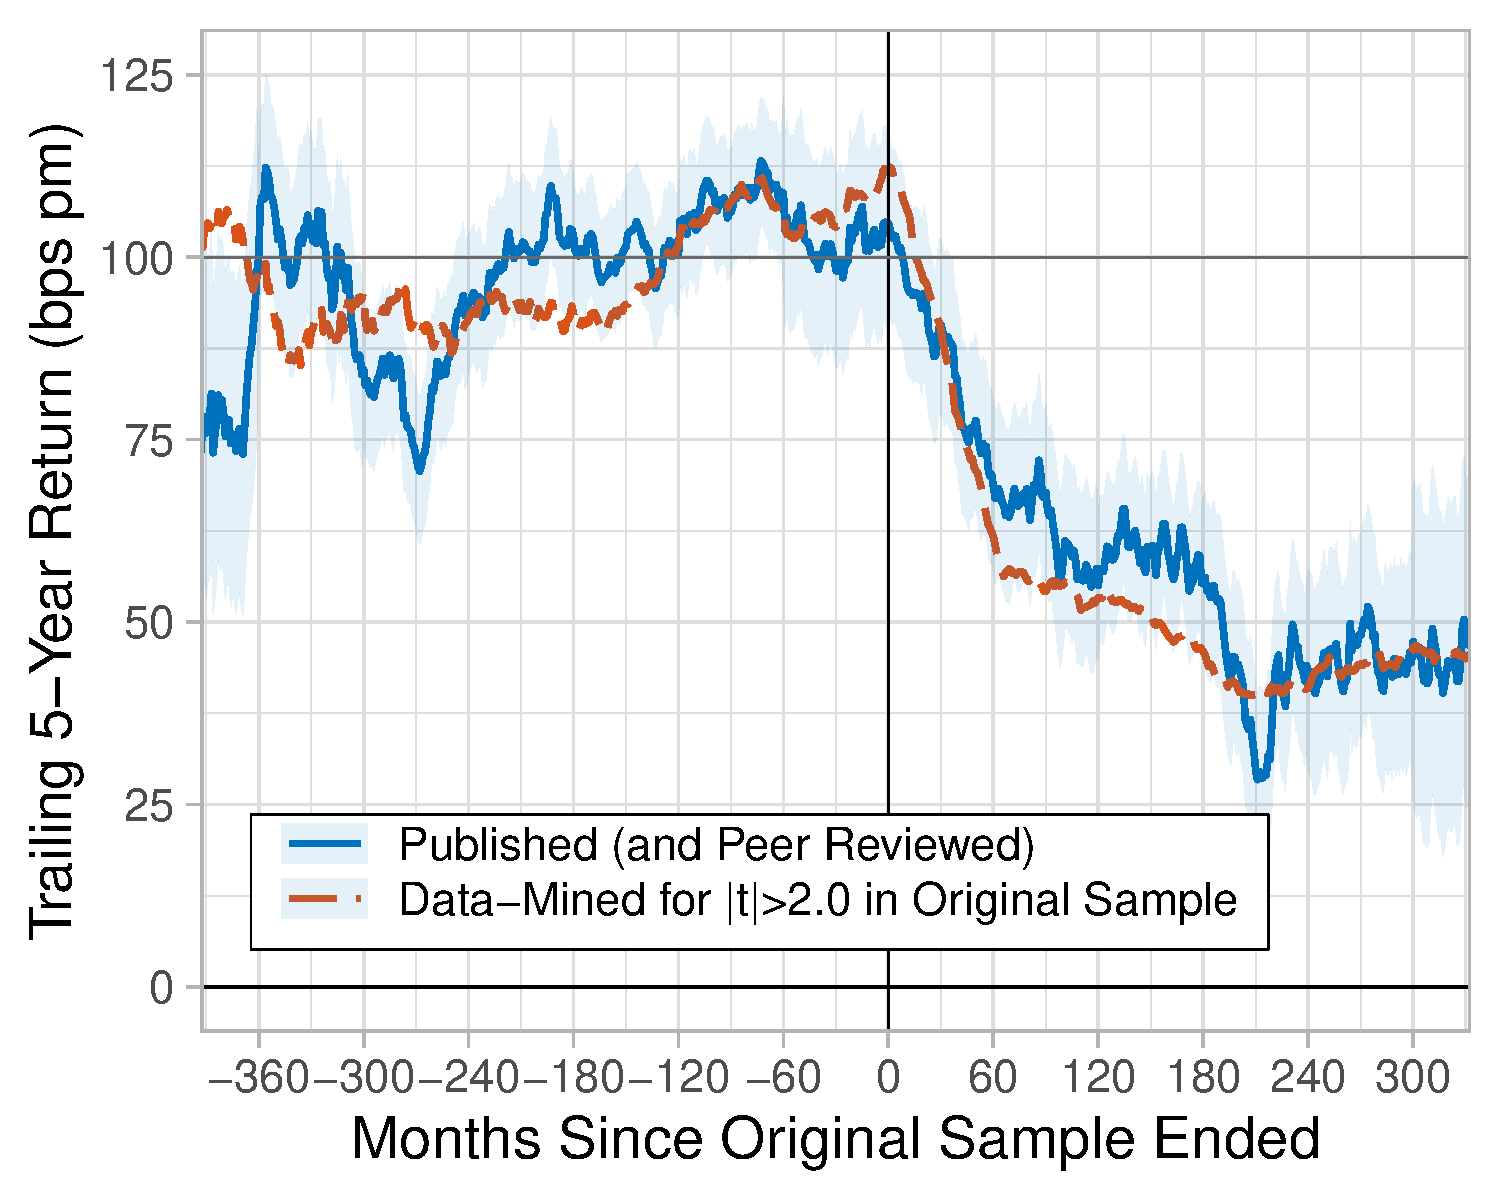
\includegraphics[width=0.7\textwidth]{exhibits/Fig_DM_t_min_2_se_indicators_calendar.pdf} 
\end{figure}

Post-sample, the performance of both types of predictors decays to about 50\% of the original sample means. Data-mined returns decay a bit more than the published returns but the difference is small, both economically and statistically. For most of the plot, the data-mined benchmark is within one standard error of the published predictors (shaded area, clustered by calendar time and predictor). We find similar results controlling for CAPM and Fama-French 3 (FF3) + momentum exposure, among many other controls. Overall, the post-sample performance of peer-reviewed and data-mined predictors is remarkably similar.

Figure \ref{fig:intro} compares the \emph{average} publication to data mining. But peer-reviewed research is heterogeneous in many dimensions, including theoretical foundations, academic discipline (finance or accounting), and journal ranking. Could this heterogeneity lead to heterogeneous outperformance compared to data mining?

To answer this question, we categorize research along the theoretical explanation for predictability (risk, mispricing, or agnostic), equilibrium modeling (no model, stylized, dynamic, or quantitative), academic discipline (finance or accounting), and journal ranking (top 3 finance, top 3 accounting, other). These categorizations are made manually, by reading the papers. Quotes that justify our classifications are in our GitHub repository.\footnote{Research categories and justifications are found at \url{https://github.com/chenandrewy/flex-mining/blob/main/DataInput/SignalsTheoryChecked.csv}.} 

Based on manual reading, peer review attributes 60\% of findings to mispricing and 20\% to risk. For the remaining 20\%, peer review is agnostic about the theoretical explanation. The low prevalence of equilibrium modeling is consistent with mispricing being the most common explanation. 15\% of peer-reviewed predictability findings are supported with an equilibrium model of any sort. 

Of the 11 research categories, only research that is agnostic about the theoretical origin of predictability shows consistent outperformance compared to data mining. But even for this category, the outperformance is sensitive to the performance metric and modest overall. In terms of post-sample FF3 + momentum alphas, agnostic research retains an additional 31 percentage points of its original-sample performance compared to data mining. But this improvement falls to 9 p.p. when using raw long-short returns. While 31 p.p. may appear notable, it is the largest outperformance out of 33 estimates, and should be shrunk toward the average of about zero to account for multiple comparisons (e.g. \citealt{chen2020publication}).

Research that takes a stand on the theoretical origin of predictability shows little, if any, outperformance. In half of our tests, research that takes a stand \emph{under}performs data mining.

Additionally, we investigate whether predictability studied in \citet{fama1992cross} (B/M), \citet{jegadeesh1993returns} (momentum), and \citet{banz1981relationship} (size) outperform data mining. These findings are not only among the most renowned, but are arguably the ones with the strongest supporting evidence, both theoretical  (e.g., \citealt{gomes2003equilibrium}; \citealt{hong1999unified}; \citealt{berk1995critique}), and empirical (e.g., \citealt{fama1993common}; \citealt{asness2013value}). Despite this supporting evidence, the post-sample performance of these findings is on average similar to data mining.

The remainder of this section discusses implications and related literature. Section \ref{sec:dm} characterizes the data mining process. Section \ref{sec:pubvs} compares the average peer-reviewed predictor with data-mining. Section \ref{sec:hetero} examines heterogeneity in research methods, including theoretical foundations. Section \ref{sec:app-most-famous} compares \citet{fama1992cross}, \citet{jegadeesh1993returns}, and \citet{banz1981relationship} with data mining. Section \ref{sec:conclusion} concludes. Robustness is in the Appendix.

\subsection*{Implications and Relation to Literature}

% put all of the interpretations here, after we establish the main empirical results
% focus on lit for likely referees
The statistical implication is straightforward: Whether a trading strategy is found in a journal or is data mined has little effect on mean inferences about post-sample performance (Equation \eqref{eq:painfully_clear}). But a closer look leads to four deeper implications.

% since this implication is very in-your-face, carefully walk through the logic.
\textit{1. Predictive Content of Empirical vs Theoretical Evidence.} 
While the peer-reviewed predictors are supported by modern empirical and theoretical evidence, the data-mined predictors combine modern empirical evidence with the most basic of financial theories: that accounting ratios may predict firm performance. This idea goes back to the 1930s (\citealt{horrigan1968short}),%
\footnote{% highlight the conceptual contrast
Some accounting ratios go back to the 1890s, but \citet{horrigan1968short} credits \citet{wall1919credit} for inspiring a ``virtual explosion of publications on the subject of ratio analysis.'' By the 1930s, there were several studies of ratios' predictive content, including \citepos{smith1935changes} study of 21 ratios.} %
decades before the modern ideas of risk, psychology, and frictions that inform the peer-reviewed predictors. Comparing the post-sample performance of peer-reviewed and data-mined predictors, then, gives a sense of the relative importance of the two types of evidence. We provide a model of this comparison in Appendix \ref{sec:app-model}.

% mention that at least some of the theories are rigorous in the modern sense.
Our estimates imply that empirical evidence is more informative than theoretical evidence for identifying stable cross-sectional predictability. Having the support of modern, peer-reviewed theory does not predict higher post-sample performance compared to using the most basic of financial theories. This result applies to all types of theory in the CZ dataset, including quantitative equilibrium models, which are typically considered the gold standard. In contrast, modern empirical evidence appears to be a requirement for post-sample robustness. Indeed, the only type of research that consistently outperforms data mining is atheoretical research, which likely provides unusually strong empirical evidence, to make up for the lack of theory. 

A priori, the importance of empirics vs theory is unclear. Some argue that theory is important (\citealt{cochrane2009asset}; \citealt{harvey2017presidential}; \citealt{fama2018choosing}), motivated by concerns about data mining bias. This concern is compelling given the volatility of stock returns and the vast number of potential predictors. However, the flexibility of theory and ``model dredging'' may limit the helpfulness of theory (\citealt{sonnenschein1972market}; \citealt{fama1991efficient}). Even if theory does identify true predictors, it may identify unstable disequilibrium phenomena that decay with investor learning (\citealt{cochrane1999portfolio}; \citealt{mclean2016does}). These previous works discuss the question theoretically, but they do not empirically compare predictors with varying amounts of theoretical support.

% start with the McLean-Pontiff framework, which it seems is quite agreeable. This is important for this takeaway, since it's quite aggressive.
\textit{2. Investors' Learning from Academic Research.} Previous papers suggest that investors learn about mispricing from academic research. If this were the case, then investors would respond to academic findings by trading on academic strategies, decreasing predictability post-sample. Consistent with this hypothesis, \citet{mclean2016does} find predictability does decay, and more so than could be explained by statistical artifacts. Post-sample changes in trading activity also support this hypothesis (\citealt{mclean2016does}; \citealt{calluzzo2019anomalies}; \citealt{mclean2020taking}). These findings beg the question of whether investors learn about risk. 

Our results suggest that learning is asymmetric: while investors learn about mispricing from academic research, they do not seem to learn about risk. Following the logic of \citet{mclean2016does}, if investors learn about risk, one would see the opposite post-sample effect: investors would avoid academic risk-based strategies, increasing predictability post-publication. We find no evidence supporting this hypothesis and strong evidence against it.

It is possible that investors do learn about risk from academic research, but that these risks decay post-sample in a manner similar to mispricing-based and data-mined predictors. In our view, the simpler explanation is that the risks identified by academic research are not considered risks by investors. This explanation is consistent with survey evidence (\citealt{doran2007really}; \citealt{mukhlynina2020choice}; \citealt{chinco2022new}; \citealt{bender2022millionaires}).

\textit{3. Effectiveness of Data Mining.} Our findings imply that data mining is surprisingly effective for identifying true cross-sectional predictability. Indeed, data mining is competitive with the peer-review process in terms of effectiveness. 

These results add to the debate that began with \citepos{yan2017fundamental} pioneering study of 18,000 accounting ratios and 4,000 past return signals.\footnote{% begin footnote
Earlier studies by \citet{ou1989financial}, \citet{abarbanell1998abnormal}, and \citet{haugen1996commonality} successfully predict cross-sectional returns using many accounting signals. But they consider far fewer signals (up to 68) and do not focus on data mining bias.
} % end footnote
Yan and Zheng reject the null of no predictability based on both bootstrap and out-of-sample tests. However, followups to Yan and Zheng come to contradictory conclusions, based on technical statistical methods (\citealt{Chordia2020Anomalies}; \citealt{harvey2020false}; \citealt{chen2024most}; \citealt{gotofalse}). Our simple data mining process and straightforward out-of-sample tests help provide clarity to this debate.

More broadly, the literature on data mining goes back to \citet{Jensen1970Random}. Earlier studies focused on statistical theory (\citealt{Lo1990Data}) or market timing (\citeauthor{sullivan1999data} \citeyear{sullivan1999data}, \citeyear{sullivan2001dangers}), and found mixed results regarding effectiveness. Other recent studies examine cross-sectional predictability indirectly, using published predictors. Most of these studies find that data mining biases are small (\citealt{mclean2016does}; \citealt{chen2020publication}; \citealt{Jacobs2020Anomalies}; \citealt{jensen2022there};  \citealt{chen2025t}), though a few argue for sizeable biases (\citealt{harvey2016and}; \citealt{hasler2023looking}). By directly examining data-mined predictors, we obtain cleaner inferences. Following up on our paper, \citet{chen2023high} and \citet{marrow2024real} use empirical Bayes to mine data more rigorously. 


\textit{4. Risk vs Mispricing in the Cross-Section.} Our findings are consistent with the view that mispricing is the primary driver of cross-sectional stock return predictability. We find that peer review is three times more likely to attribute predictability to mispricing than to risk. Moreover, predictors attributed to risk decay post-sample.

% what do other papers find?
These findings complement recent papers that also point toward mispricing as the primary driver. These papers use a wide range of methods, including announcement effects (\citealt{Engelberg2018Anomalies}; \citealt{frey2023stock}), stochastic dominance (\citealt{holcblat2022anomaly}), machine learning (\citealt{bali2023expected}), and subjective expectations data (\citealt{jensen2024subjective}). 



% ===================
